\chapter{Advertising: Handling Abrupt Phases}

The object of this section is the design a sliding-window combinatorial bandit algorithm for optimizing the budget allocation over the three sub-campaigns in order to maximize the total number of clicks, in the case in which there are the three abrupt phases.
For addressing this assignment \ref{assPart3} we started from the simplified case of one single phase solved in the previous section and we extended it in order to take in consideration the more general scenario of multiple phases.\\

\section{Sliding window mechanism}
For this purpose we have implemented the \textit{AbruptBiddingEnvironment.py} class which extends the \textit{BiddingEnvironment.py} class. This class works in a scenario of multiple abrupt phases by returning, for each sub-campaign, the reward of a given pulled arm, depending on the phase we are in.

In this case, the functions generating  the number of clicks given a bid value can change dynamically, according the phase we are in.
The curves differ from the previous definitions only for the dependence to the phase we are in. As follows the mathematical defintion of the three curve functions:

\begin{equation}
	n(x) = c_{M}[phase] \cdot (v_{M}[phase] - e^{-\alpha x})
\end{equation}

In order to learn the three curves in the case of multiple abrupt phases, we have implemented the \textit{DynamicLerner.py} class as an extension of the standard GP\_Learner.
It implements a \textit{sliding window} mechanism in which we pull a new arm and add the collected rewards until the length of the window is reached. When the window is full, for each new pulled arm we get, we delete the last recent value and add the new one to the collected rewards.

\section{Changes Detection mechanism}

For solving this problem we have implemented an innovative method which is based on the concept of the \textit{Statistical test}.
We recall that a statistical test is a procedure for deciding whether a hypothesis about a quantitative feature of a population is true or false. Then for testing a hypothesis, we draw a random sample and calculate an appropriate statistic on its items. If, in doing so, we obtain a value of the statistic that would occur rarely when the hypothesis is true, we would have reason to reject the hypothesis.

In our scenario, to detect changes, we need to compare the value of the new drawn sample with the distribution of the points belonging to the same arm in order to decide whether the hypothesis $H_0$,that the new drawn point belongs to that distribution, is true.
Let us suppose to draw a sample whose value is $x_0$ and let $\mu$ $\sigma^2$ be respectively the average
and the standard deviation of the the distribution of the points belonging to the pulled arm. 
If the point doesn't belong to that distribution the hypothesis test should reject $H_0$, with a \textit{confidence interval of 99\%} So we have:

\begin{equation}
	 \mathbb{P}\left(\frac{|x_0 - \mu|}{\sqrt{\sigma^2}} > h \right) = 0.01
\end{equation}

We have that the critical z-score when using a 99\% confidence level are $\pm 2.58$ standard deviations.\\

In the \textit{DLChangeDetect.py} class, we have implemented such change detector. When an arm is pulled more than '\textbf{min\_len}' \footnote{min\_len indicates the minimum number of data we considering in an arm} times, for each pull we run the statistical test. When the test reject $H_0$, it means that the point doesn't belong to that distribution and so it means that it is changed. In this case we reset the arm.\\ 

\section{Performance evaluation}

In Figure \ref{regretPart3Fig} a comparison of the performance of three algorithms \footnote{Combinatorial bandit algorithm without sliding window, Combinatorial bandit algorithm with sliding window and Change detection
implementation} is shown. As before, for the performance evaluations we have computed the \textit{cumulative regret} as the difference between the expected reward of the \textit{Clairvoyant algorithm} and the expected reward of the implemented algorithms. 
\begin{figure}[!htb]
	\centering
	%\captionsetup{justification=centering,margin=1cm}
		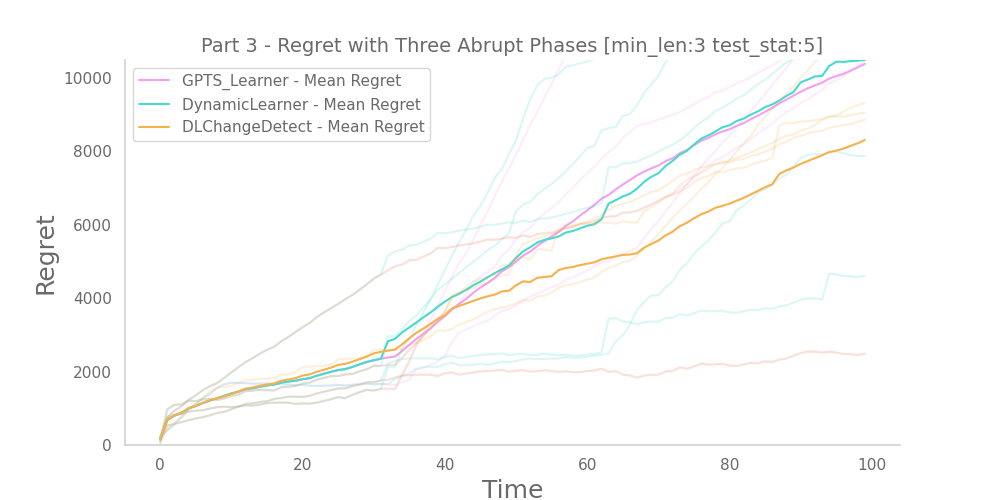
\includegraphics[width=\textwidth]{images/part3_min-len3_test-stat5.png}
	\caption{Cumulative regret in scenario with multiple abrupt phases}.
	\label{regretPart3Fig}
\end{figure}
